\subsection*{Runtime Efficiency}\label{subsec:runtime}
A consideration in a compiler is the performance or efficiency of its output. 
Rather than blindly translating the source code, translating to something more efficient is a subproblem in compiler optimization.
Optimization is however a nonspecific and subjective word, therefore in \gls{gamble} we will instead be referring to the problem as runtime efficiency.
Runtime efficiency entails considerations of memory allocation, pipelining, parallelization etc. which may have an impact on execution time.
To do an efficient and complete analysis of how to increase runtime efficiency, information of the situation in program is required.
This is where \gls{gamble} is at a disadvantage. 
\gls{gamble} distances its programmers from controlling where the code is performed and instead does so seamlessly.
Information about how e.g. a for-loop could be transformed into a kernel does not exist in \gls{gamble} which makes it difficult to do this.
The seamless use of the \acrshort{gpu} means that information is lackluster and therefore all computations may not be candidates for improving its runtime efficiency, this is one of the trade-offs \gls{gamble} makes, meaning that simplicity is valued over performance.
If \gls{gamble} were to require more information, e.g. whether or not something is parallelizeable or ask the programmer to determine what type of memory on the \gls{gpu} should be used for each variable, the simplicity and seamless use of the \acrshort{gpu} would be lost.

As previously mentioned due the object code being OpenCL C certain considerations pertaining to instruction handling and register allocation etc. are not of interest for this compiler.
This is handled by using another compiler to compile the OpenCL C code into machine code, see \todo{REF TIL MAKEFILE}. 
Instead to increase runtime efficiency the considerations instead pertain to when the \acrshort{gpu} should be used.

As \gls{gamble} is attempting to seamlessly use the \acrshort{gpu} to increase performance, knowing when the use of the \acrshort{gpu} will actually be beneficial is an important point in the code generation process.
As mentioned to do this efficiently, the compiler would require more information about the computations which are to be performed, than can be read from the syntax of \gls{gamble}.
Therefore it is decided that it is better to be sure that a computation can benefit from the \acrshort{gpu}, rather than risking moving computations that wont benefit with those that will.
As such only those operations that the project group knows have a possibility of benefiting from the parallel abilities of the \acrshort{gpu} will be executed on the \acrshort{gpu}. 

%Knowing when to use GPU
Even though a computation can be parallelized, does not necessarily mean it should be moved to the \acrshort{gpu}, as is evident in \myref{image:benchmark}.
This is an opportune moment for improving the runtime efficiency of the object code by using the \acrshort{gpu} only when it will be superior than the \gls{cpu} in regards to performance.
A possibility of doing so would be to analyze whether or not an instruction sequence both entail a sufficient amount of operations and that these are not sequentially dependent on each other.
Performing such an analysis increases compile time.
Because of the difficulty to discern not only if there will be an actual increase, but also if any custom functions created by the programmer are fit to run on the \acrshort{gpu} this analysis is not part of the \gls{gamble} compiler.
Instead only vector and matrix operations already defined in the language, by having an operator, will be performed on the \acrshort{gpu}.

%Optimising OpenCL Kernals
A function that is to be run on the \acrshort{gpu} is in the OpenCL framework called a kernel.
Since kernel code uses explicit memory handling, one must choose what memory space on the \gls{gpu} to allocate ones variables in as well as using the principle of locality.
This can provide a substantial (more than 3 times) faster runtime. \citep{ocl_lecture3}
\begin{figure}[h]
\centering
 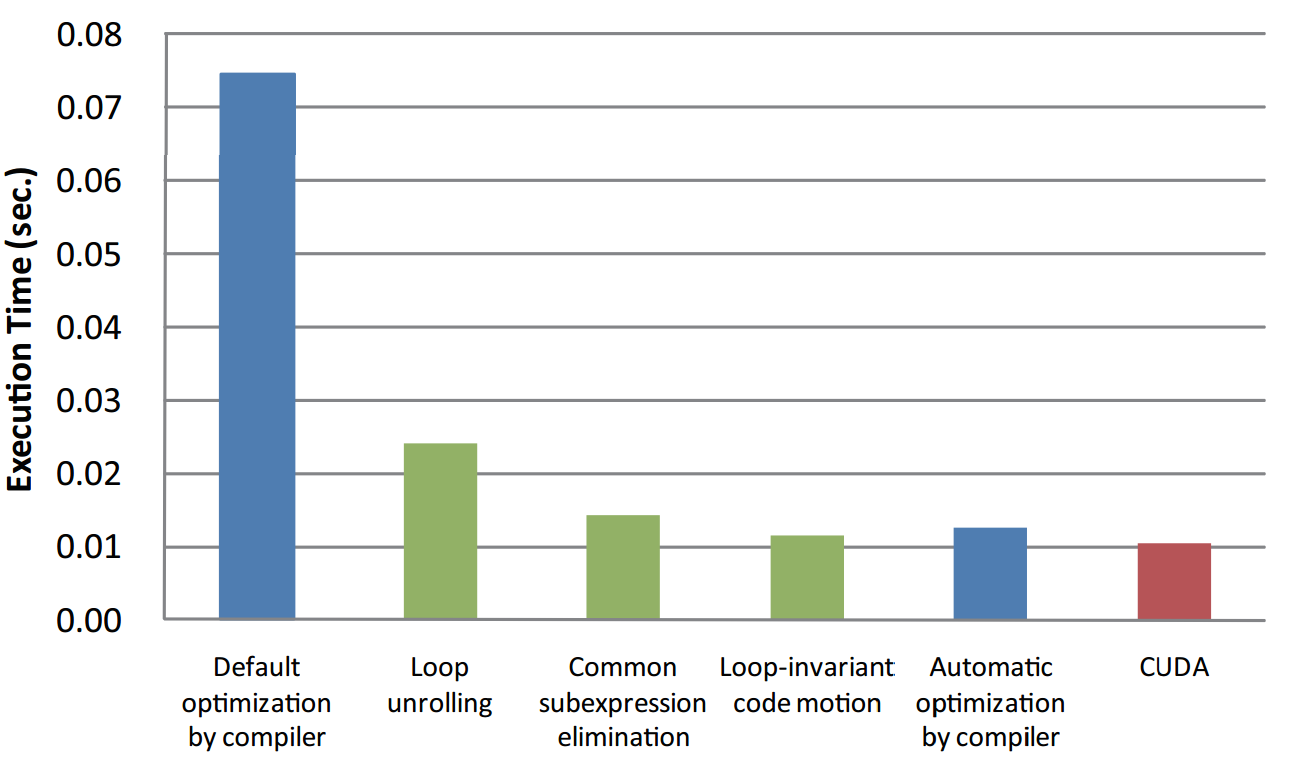
\includegraphics[width=1\textwidth]{figures/opencloptimisation.png} % trim=4.85cm 15cm 0.85cm 1cm
\caption{Execution speed of a matrix multiplication with different optimizations done. \citep{CUDAOpenCLOptimisation}}\label{image:OpenCLOptCompare}
\vspace{-15pt}
\end{figure}
As seen on \myref{image:OpenCLOptCompare} some possible methods of increasing runtime efficiency includes loop unrolling, common sub-expression elimination and loop-invariant code motion. 
These are taken as specific examples in this comparison because these methods are performed in the \acrfull{ptx} code that CUDA compiles to. %ENDING A SENTENCE WITH A PROPOSITION OMG!!!
An OpenCL C compiler will also optimize the source code if given the instruction to, however its impact depends on the \gls{gpu} and platform in use.
The value of any optimization is situational, i.e. changing the work-group size can yield improvements of up to 5 times. \citep{ocl_lecture3}
OpenCL can use just-in-time compilation to generate binary code to the appropriate device it is working with at runtime.
This allows OpenCL to optimize for the \gpu{gpu} used, however this is also a constant overhead for each execution of the program. 
OpenCL can also compile the kernels before runtime, this is known as an offline compilation as opposed to the just-in-time compilation known as online. 
The CUDA compiler \texttt{nvcc} is a two step process, which first generates \acrshort{ptx} bytecode and then either JITs on runtime or compiles a so called ``fat binary'' at compile time, which contains multiple programs for different \gls{gpu}s. \citep{nvidia_cude_fat_bin}

%Optimising C code(CPU)
As \gls{gamble} does not exclusively perform its operations on the \acrshort{gpu} the code run on the \acrshort{cpu} must also be considered as a point in which runtime efficiency can be increased.
Some methods of increasing runtime efficiency on the \acrshort{cpu} are similar as mentioned earlier such as loop unrolling.
Further methods pertain to the architectural differences between \acrshort{cpu}s and \acrshort{gpu}s, in particular cache- and pipeline-friendly code.
Cache-friendly code means considering the principle of spatial locality i.e. memory regions closer to each other, are more likely to be accessed within a short time.
To write pipeline-friendly code one must in particular consider branch prediction, however the best way is simply to avoid branching. \citep{CCodeOpt}
While these methods may very well increase runtime efficiency, there is no reason to implement them as the GNU Compiler Collection already implements well developed methods of increasing runtime efficiency beyond our abilities.
